\documentclass{article}
\usepackage[utf8x]{inputenc}

\usepackage{booktabs}
\usepackage{caption}
\usepackage{eurosym}
\usepackage{graphicx}
\usepackage{float}
\graphicspath{ {images/} }
\usepackage[margin=1in]{geometry}

\begin{document}
\begin{center}
    \large{Construção de um motor DC}\\
    2016--2017
\end{center}
\centering
\begin{tabular}{ccc}
    Bernardo Meurer & Maria Adelaide Ambrósio & Inês Coelho\\
    86242 & 87064 & 87022
\end{tabular}
\vfill
\begin{table}[H]
\centering
\begin{tabular}{@{}ll@{}}
\toprule
Tarefa      & Tempo Gasto \\ \midrule
Planeamento & 20min       \\
Compra      & 120min      \\
Construção  & 65min       \\
Testes      & 15min       \\ \midrule
Total       & 220min
\end{tabular}
\hskip 30pt
\centering
\begin{tabular}{@{}ll@{}}
\toprule
Peça      & Custo \\ \midrule
Íman      & 1,60€ \\
Pilha     & 4,00€ \\
Terminais & 1,50€ \\
Fio       & 0,50€ \\ \midrule
Total     & 7,60€
\end{tabular}
\end{table}

\begin{figure}[H]
    \centering
    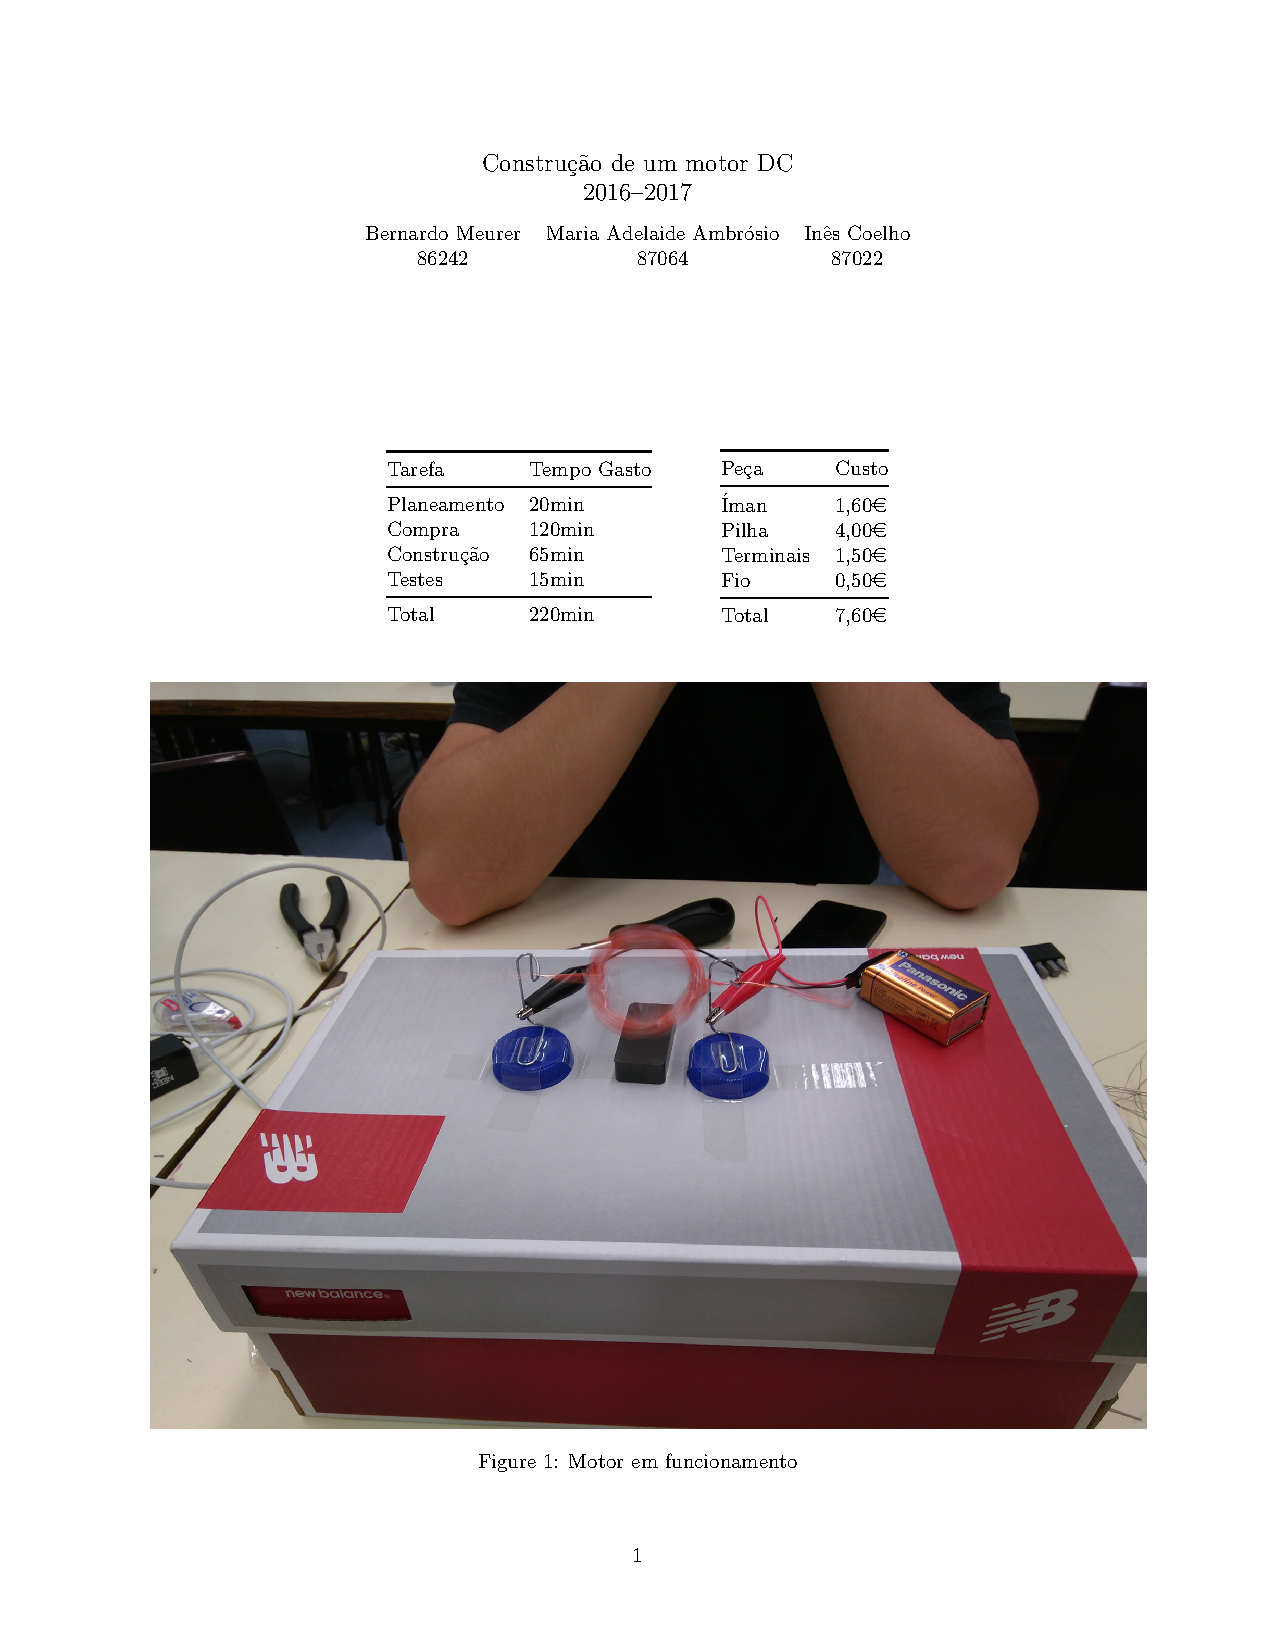
\includegraphics[scale=.25]{motor}
    \caption{Motor em funcionamento}
\end{figure}

\end{document}
